The aim of this project was to develop a computer graphics application combining several state-of-the-art techniques into a beautiful world. 
\begin{figure}[H]
  \centering
  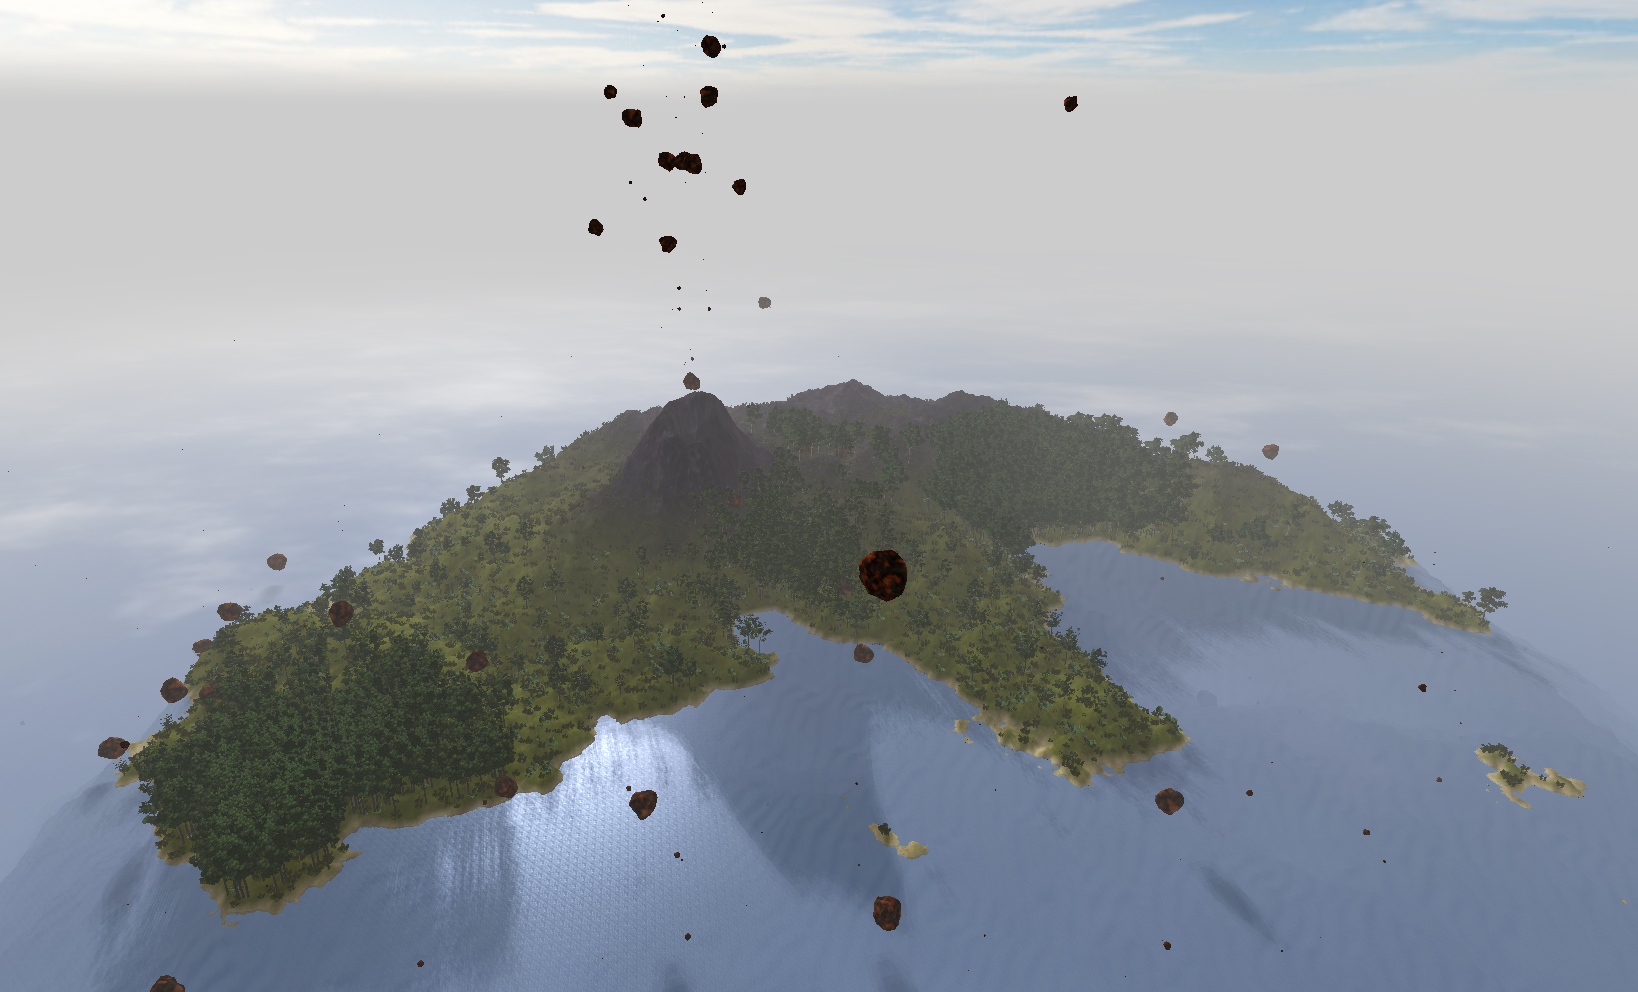
\includegraphics[width=1.0\linewidth]{images/frontImage.jpg}
  \caption{A beautiful world. Contarining 3000 trees and 13000 bushes, and a terrain with a vertex density of 5.5.}
  \label{fig:beautifulIsland}
\end{figure}%

TODO: List of what we have done? (e.g. det som var på sliden som vi började vår presentation med.)?


The project was performed as a part of the course TSBK03 - Techniques for advanced computer games. The code is written in C++11 and GLSL version 150. We use Qt 5.1 as OpenGL wrapper and context provider and OpenCV for some mathematical operations and filtering.